\chapter{Diseño del experimento}
En este capítulo se analizan los resultados que se obtuvieron al haber implementado el modelo, y se divide en tres partes.
En la primera de ellas se cuenta cómo es que se decidió implementar el modelo, así como también cuales de sus variables se dejaron fijas (serían constantes en esta implementación) y cuáles es posible variar desde la interfaz de usuario.

En la segunda parte se diseñaron ciertas pruebas con el fin de poner en evidencia características particulares del modelo, específicamente su correcto comportamiento físico.

Y en la última parte se reportan los resultados de las pruebas de desempeño a las que se sometió el programa.

\section{Definición del sistema}
En esta primera parte presento el experimento y explico que parámetros fijé y cuáles pueden ser cambiados por el usuario.

\subsection{Características del modelo}
Tal como se explicó en la Sección~\ref{descripcion:experimento}, se modela un hexaedro regular, donde cinco de sus seis caras son rígidas y la cara superior o tapa es flexible: además, asumo que este hexaedro está relleno de gas.
En este sentido, el hexaedro completo (o caja) es el cuerpo neumático.
Mientras que la cara superior (o tela) es el cuerpo flexible.
Se deja caer sobre la tela una esfera rígida (o pelota).
Un ejemplo del programa terminado se muestra en la Figura~\ref{programa:portada}.
\begin{figure}
 \centering
 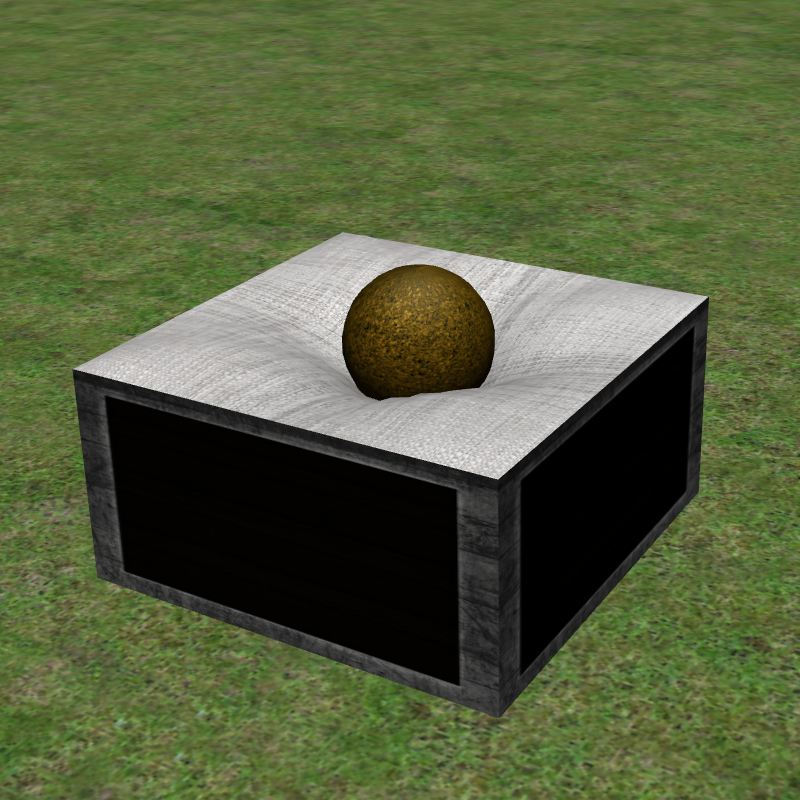
\includegraphics[width=0.85\textwidth]{Img/04/modeloPortada}
 \caption[Ejemplo del programa en ejecución]{Una imagen del programa que implementa el modelo.}
 \label{programa:portada}
\end{figure}

\subsubsection{Constantes del experimento}
En una situación como la antes descrita hay muchísimas variables del modelo, sin embargo al momento de hacer la implementación en código decidí dejar fijas algunas de ellas, es decir que la única manera de cambiarlas es modificando en el código fuente y recompilando el programa por completo.
Aquí está la lista de estas variables y su significado.

Las variables que se decidieron dejar fijas, y que por ende se convierten en constantes en el experimento son las siguientes:

\begin{itemize}
 \item El número de partículas por lado de la tela.
 \item Las dimensiones (alto, ancho y largo) de la caja.
 \item La masa total de la tela. Y por lo tanto, la masa de cada partícula es ésta cantidad dividida entre el número total de partículas.
 \item El radio y la posición de la pelota.
 \item El tamaño del paso en el tiempo $\Delta t$ que se usa para los métodos numéricos de integración.
\end{itemize}

Los valores de estas constantes con las que se hizo este experimento están en el Cuadro~\ref{valores:constantes}.
\begin{table}
\ra{1.2}
\begin{center}
\begin{tabular} {@{}lrp{8cm}@{}}
\toprule
Constante & Valor & Comentario\\ 
\midrule
 Número de partículas & 22 & Para que se vea mejor el modelo, se elige un número par\\
 Dimensiones caja & $0.75 \times 1.5 \times 1.5$ & Se forma una caja de tapas cuadradas \\
 Masa tela & 10 & La masa de cada partícula es entonces $\frac{10}{22^{2}}$ \\
 Radio pelota & 0.25 &  \\
 Posición pelota & $(0, 1.5, 0)$& Como el cuerpo neumático está centrado en el origen. La pelota está justo arriba de él en el centro\\
 $\Delta t$ & 0.0025 & Determinado experimentalmente \\
\bottomrule
\end{tabular}
\caption[Valores de las constantes durante el experimento]{Valor de las constantes del experimento}
\label{valores:constantes}
\end{center}
\end{table}

\subsubsection{Variables físicas del experimento}
La variables físicas del experimento pueden ser modificadas en tiempo de ejecución por medio del menú que muestra en la Figura~\ref{programa:menu}.

\begin{figure}
 \centering
 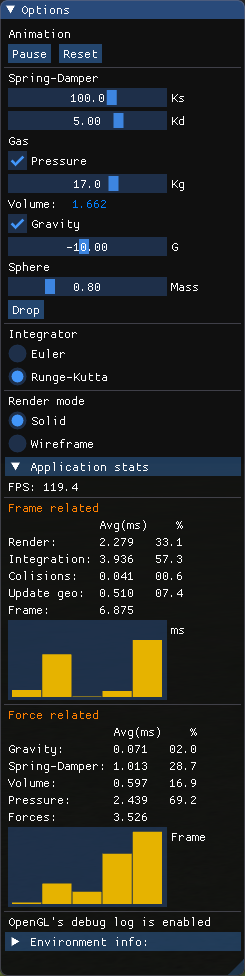
\includegraphics[width=0.33\textwidth]{Img/04/menu}
 \caption[Menú de usuario del programa]{Menú de usuario.}
 \label{programa:menu}
\end{figure}

Para la pelota o esfera (\emph{\textenglish{Sphere}}) que se refiere al cuerpo rígido.
la única variable que se puede modificar es su masa.

Los parámetros del cuerpo flexible que es posible modificar se dividen en tres subcategorias una por cada fuerza que se acumula.

La categoría del \emph{Gas}, al que se puede prender o apagar por medio del checkbox \emph{\textenglish{Pressure}}. 
Además, se puede modular su magnitud variando el valor de la constante $k_{g}$, por medio del control.

La de la \emph{\textenglish{Gravity}}, que al igual que la anterior se puede prender o apagar con el control  y también se puede modular variando el valor de la constante $g$.

La última subcategoria es la debida al resorte amortiguador (\emph{\textenglish{Spring-Damper}}.)
Esta fuerza no se puede apagar, pero se puede variar modificando dos parámetros $k_{s}$, que, como ya se dijo, controla la rigidez del resorte y $k_{d}$ que controla el amortiguamiento o pérdida de energía debida al resorte.

Aunque no es propiamente una opción de la física. El menú también permite elegir que método numérico usar para integrar.
Las opciones disponibles son: \emph{Euler} y \emph{Runge-Kutta}.

Los valores de default de estas variables (el valor que tiene al iniciar la ejecución) son los que muestra la Tabla~\ref{valores:variables}.

\begin{table}
\ra{1.2}
\begin{center}
%\begin{tabular} {|c|c|p{10cm}|}
\begin{tabular} {@{}llp{10cm}@{}}
\toprule
Parámetro & Valor & Comentario\\
\midrule
 Masa & 0.08 & Masa del cuerpo rígido \\
 Integrador & Runge-Kutta & Método Numérico con el que se integra. \\
 Gas & Activado & El programa empieza con la fuerza del gas prendida \\
 $k_g$ & 17 & Constante de presión del gas \\
 Gravedad & Activada & La gravedad está activada \\
 $g$ & -10.0 & La gravedad es negativa (jala hacia abajo) \\
 $k_s$ & 100 & La fuerza de los resortes \\
 $k_d$ & 5 & El valor de damping \\
\bottomrule
\end{tabular}
\end{center}
\caption[Valores por defecto de las variables físicas]{Valor inicial de los parámetros del experimento}
\label{valores:variables}
\end{table}

\subsubsection{Opciones de control y visualización}
Hay otras opciones que se pueden modificar por medio del menú, que se refieren más a cómo controlamos la animación y a como se ve el modelo que a la física.

Dentro de las del flujo de la animación, sólo hay dos controles, el de \emph{\textenglish{Pause/Play}}, que puede detener (reanudar) la animación física (se sigue pudiendo mover la cámara).
Y el botón de \emph{\textenglish{Reset}}, que devuelve a todos los objetos a su posición original.

El botón de \emph{\textenglish{Drop}}, hace que la esfera se deje caer.

Dentro de la categoría de \emph{\textenglish{Render}}, se encuentran las siguientes opciones:

La primera opción \emph{\textenglish{solid}}, usa el modelo de iluminación de Phong (los materiales se obtienen de texturas) para dibujar todos los objetos en la escena.

Y la segunda opción \emph{\textenglish{wireframe}}. 
Que solo cambia la manera de dibujar el cuerpo neumático.
Dibuja con lineas azules las orillas de la caja y dibuja en una escala de color entre amarillo y rojo, los resortes (como lineas) y las particulas (como puntos) que forman el cuepor flexible.
El color asignado depende de la magnitud de la fuerza que actúa sobre ellos.

Finalmente, además del menú de usuario, hay opciones que solo se pueden modificar por medio del \textenglish{mouse} y del teclado.

\begin{itemize}
 \item Arrastrar el mouse con el botón izquierdo presionado, permite modificar el ángulo de la cámara. Se usa el modelo de \emph{\textenglish{trackball camera}}.
 \item La rueda del mouse, cambia el \emph{\textenglish{zoom}} de la cámara.
 \item Presionar la tecla `\emph{s}' en el teclado toma un \emph{\textenglish{screenshot}}. Las imágenes son guardadas en el folder \mintinline{cpp}{Screenshoots} (Que debe ser creado por el usuario) en el mismo folder donde esta el ejecutable.
 \item Presionar \emph{Escape} en el teclado termina la ejecución del programa.
 \item Presionar la tecla `\emph{m}' muestra/oculta el menú de usuario.
 \item Presionar \emph{F11} cambia entre el modo de pantalla completa y de ventana.
 \item La tecla `\emph{p}' es un atajo para el botón de \emph{\textenglish{Play/Pause}} de la animación.
 \item La tecla `\emph{r}' es un atajo para el botón de \emph{\textenglish{Reset}} de la animación.
\end{itemize}

\subsection{Características del entorno de pruebas}

\subsubsection{Software}

El programa fue desarrollado en lenguaje C++ y los \emph{\textenglish{shaders}} que sirven para hacer el render fueron escritos en GLSL.

Para poder compilar el código fuente de este programa es necesario tener un entorno de programación que contemple lo siguiente:

Un compilador de C++ y las siguientes bibliotecas: OpenGL, glfw, Dear Imgui, GLM, GLEW, FreeImage y Assimp.

Todos éstos requerimientos son software libre (Más detalles de esto en el Apéndice).
Aunque este trabajo fue desarrollado en su totalidad en un sistema operativo GNU/Linux, todos los requerimientos tienen la enorme ventaja de estar disponibles en cualquier plataforma.
Si las bibliotecas están correctamente instaladas, el programa debe compilar y funcionar bajo cualquier sistema operativo.

\subsubsection{Hardware}
La mayoría de las pruebas fueron hechas en una laptop personal MSI GF65, con las siguientes características.

\begin{itemize}
\label{maquina:trabajo} 
 \item Procesador: Intel Core i7-9750H CPU @ 2.60GHz $\times$ 12.
 \item Memoria: 32GB DDR2.
 \item Tarjeta de Video: Nvidia GeForce GTX 1660 Ti Mobile\footnote{Aunque la laptop tiene la tarjeta de video descrita, el programa es tan simple que de hecho puede ejecutarse en la tarjeta de video integrada del procesador Intel sin problemas.}
 \item Sistema Operativo: Ubuntu 20.04 64 bits.
\end{itemize}

Esto no quiere decir que este sea el hardware mínimo, sólo que la \emph{mayoría} de las pruebas se realizaron en éste hardware.
Sin embargo, se ha ejecutado con éxito en equipos bastante accesibles. 
Éste trabajo es de hecho una reedición, el trabajo original se desarrolló usando una laptop convencional en el año 2008.
Actualmente, éste programa debe poder ejecutarse en cualquier computadora personal, de escritorio o equipo móvil sin problemas de capacidad del \emph{\textenglish{hardware}}.
Hoy en día la única limitante (de existir) podría acaso ser el \emph{\textenglish{software}}.

\section{Características físicas del modelo}
Para poner en a prueba la fidelidad del modelo, se hicieron una serie de pruebas.
Estas pruebas tienen dos finalidades: primero probar la sensibilidad del programa ante la variación de sus parámetros físicos y segundo comprobar cualitativamente que el fenómenos físico funciona correctamente.

\subsection{Probando la gravedad}
La gravedad es la única fuerza que actúa tanto en el cuerpo flexible como en en el cuerpo rígido. Para entender mejor cómo afecta se sugieren las siguientes pruebas.

Partiendo de los valores de \emph{\textenglish{default}}, se espera a que la tela se estabilice (Figura~\ref{fig:testGEstable}).
Ahora se \emph{aumenta} la gravedad a su valor más \emph{pequeño} (recordemos que hacer la gravedad más fuerte es hacerla más negativa), es decir, $g=-20$, se observa ahora cómo la gravedad es muy fuerte para que la presión del gas infle la tela, por lo que queda colgando un poco.
Las partículas que forman el cuerpo flexible son muy pesadas (son jaladas con más fuerza hacia abajo).
Esta situación se muestra en la Figura~\ref{fig:testGAumenta}. 
Ahora se deja caer la pelota y se espera que se estabilice de nuevo el programa, (Figura~\ref{fig:testGCae}) la gravedad hace que la pelota y las partículas pesen más, sin embargo la fuerza del gas que no se ha tocado compensa de alguna manera y no deja que se hunda más la pelota.
Con la pelota estable sobre la tela, apagué la fuerza del gas.
Al apagar la fuerza que equilibraba la gravedad todo se va hacia abajo, por la gravedad, pero como además esta fuerza es grande, la rigidez del resorte es poca para evitar un efecto de súper elongación como el que se ve en la Figura~\ref{fig:testGNoPres}, donde la pelota es detenida por el piso.

\begin{figure}
 \centering
  \begin{subfigure}[b]{0.45\textwidth}
    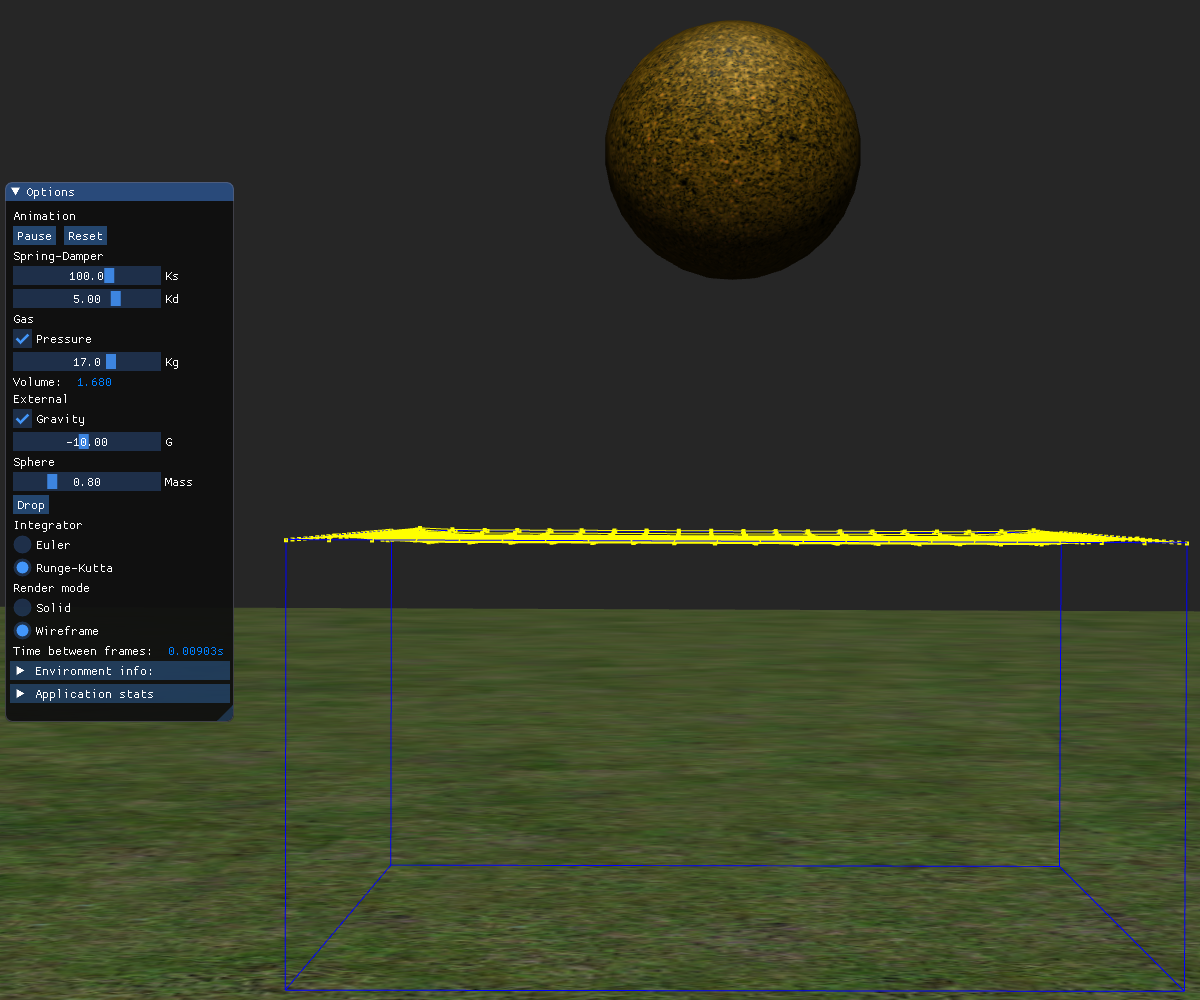
\includegraphics[width=\textwidth]{Img/04/gravity1}
    \caption{La tela se estabiliza con la gravedad y la presión.}
    \label{fig:testGEstable}
  \end{subfigure}
~
  \begin{subfigure}[b]{0.45\textwidth}
    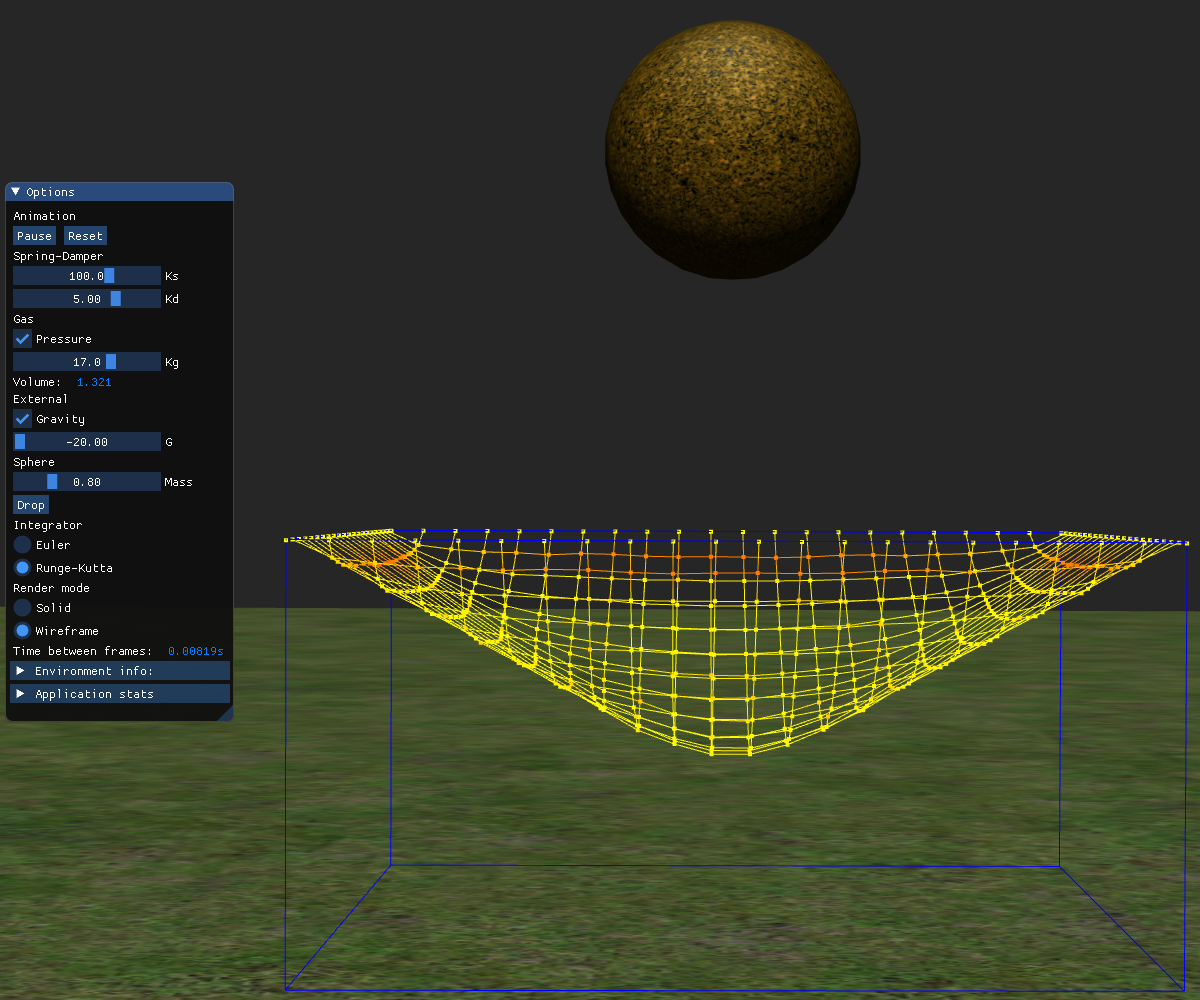
\includegraphics[width=\textwidth]{Img/04/gravity2}
    \caption{La gravedad aumenta a $g=-20$}
    \label{fig:testGAumenta}
  \end{subfigure}
\\
  \begin{subfigure}[b]{0.45\textwidth}
    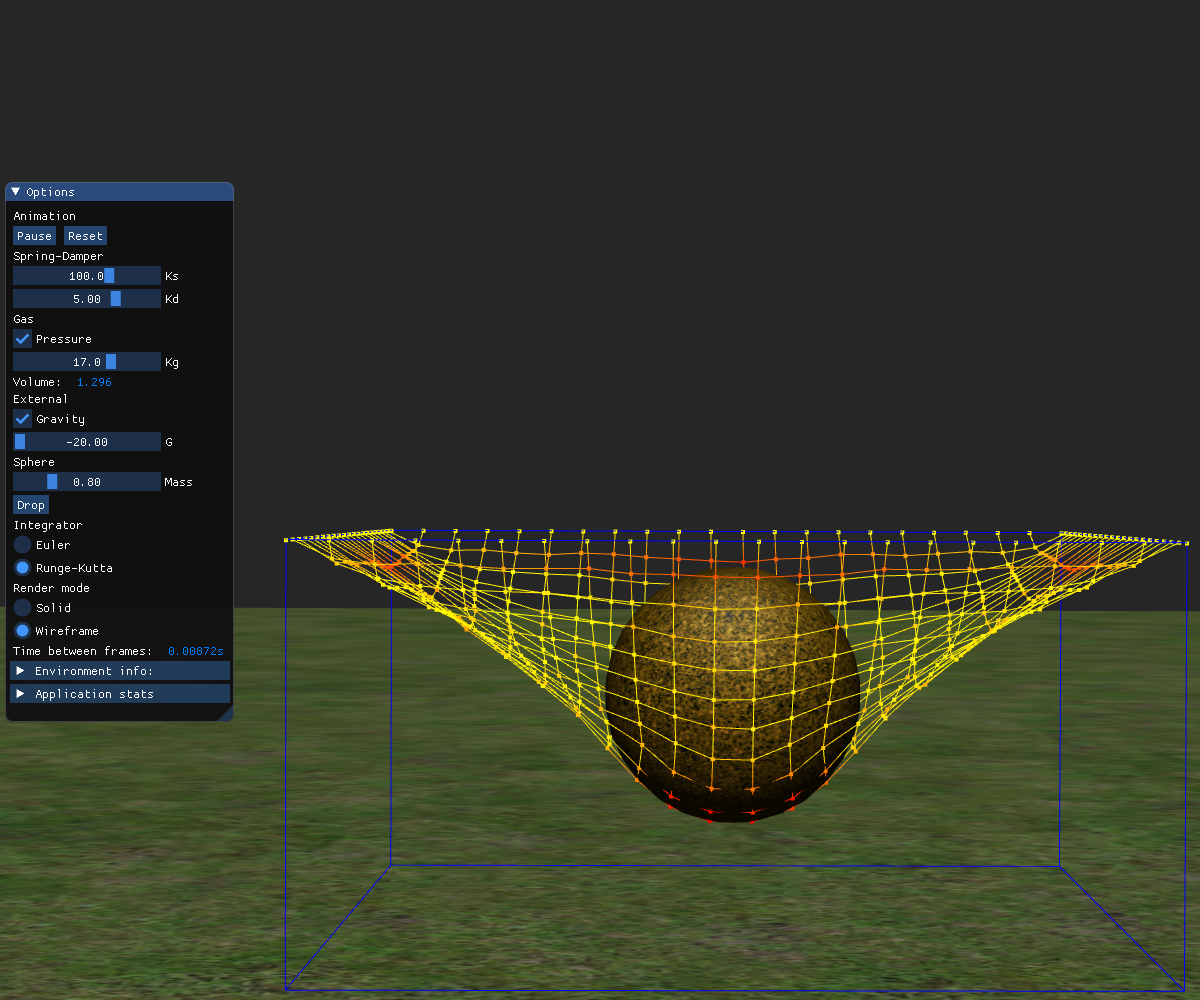
\includegraphics[width=\textwidth]{Img/04/gravity3}
    \caption{La pelota se deja caer.}
    \label{fig:testGCae}
  \end{subfigure}
~
  \begin{subfigure}[b]{0.45\textwidth}
    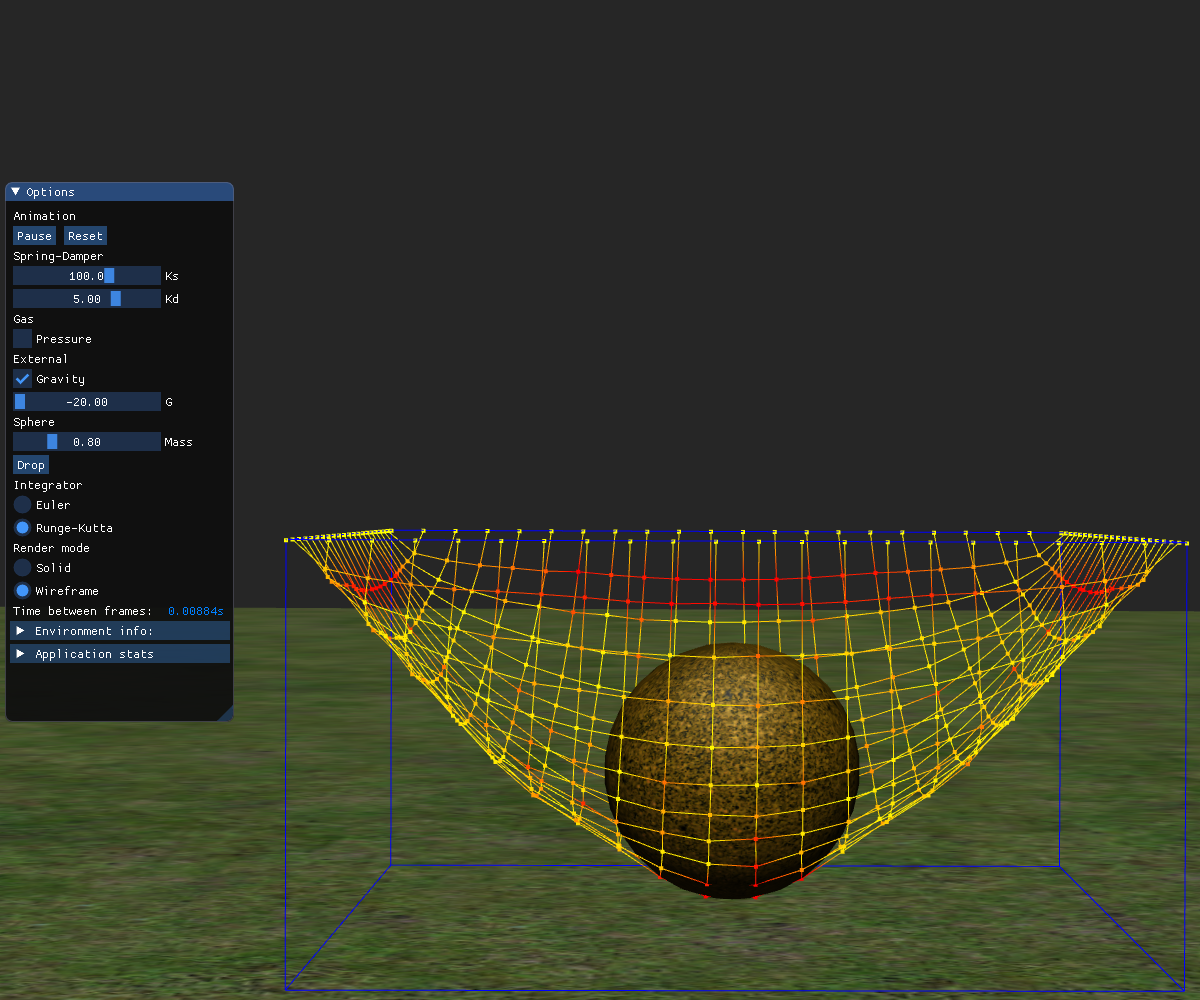
\includegraphics[width=\textwidth]{Img/04/gravity4}
    \caption{Se apaga la fuerza de presión}
    \label{fig:testGNoPres}
  \end{subfigure}
 \caption[Experimento: Fuerza de gravedad]{Probando la fuerza de gravedad} 
 \label{fig:testGravity}
\end{figure}

Reinicie la animación y vuelva a los valores de \emph{\textenglish{default}}.
De nuevo espere a que se estabilice la tela ahora disminuya la gravedad a su máximo valor posible, es decir una gravedad positiva: $g=1$.
Ahora verá que la tela se va más hacia arriba: se infla más el cuerpo flexible. 
Esto se debe a que ahora la gravedad no se opone a la presión del gas, sino más bien le favorece, por lo que el cuerpo flexible, es jalado hacia arriba aún más, como se ve en la Figura~\ref{fig:testGpos1}.
Ahora deje caer la pelota, como la gravedad es positiva y pequeña (su valor absoluto en una décima parte del valor normal) la pelota \emph{sube lentamente}, y se aleja del cuerpo flexible (Figura~\ref{fig:testGpos2}).
La constante de gravedad influye en la velocidad de caída de los cuerpos.

\begin{figure}
 \centering
  \begin{subfigure}[b]{0.45\textwidth}
    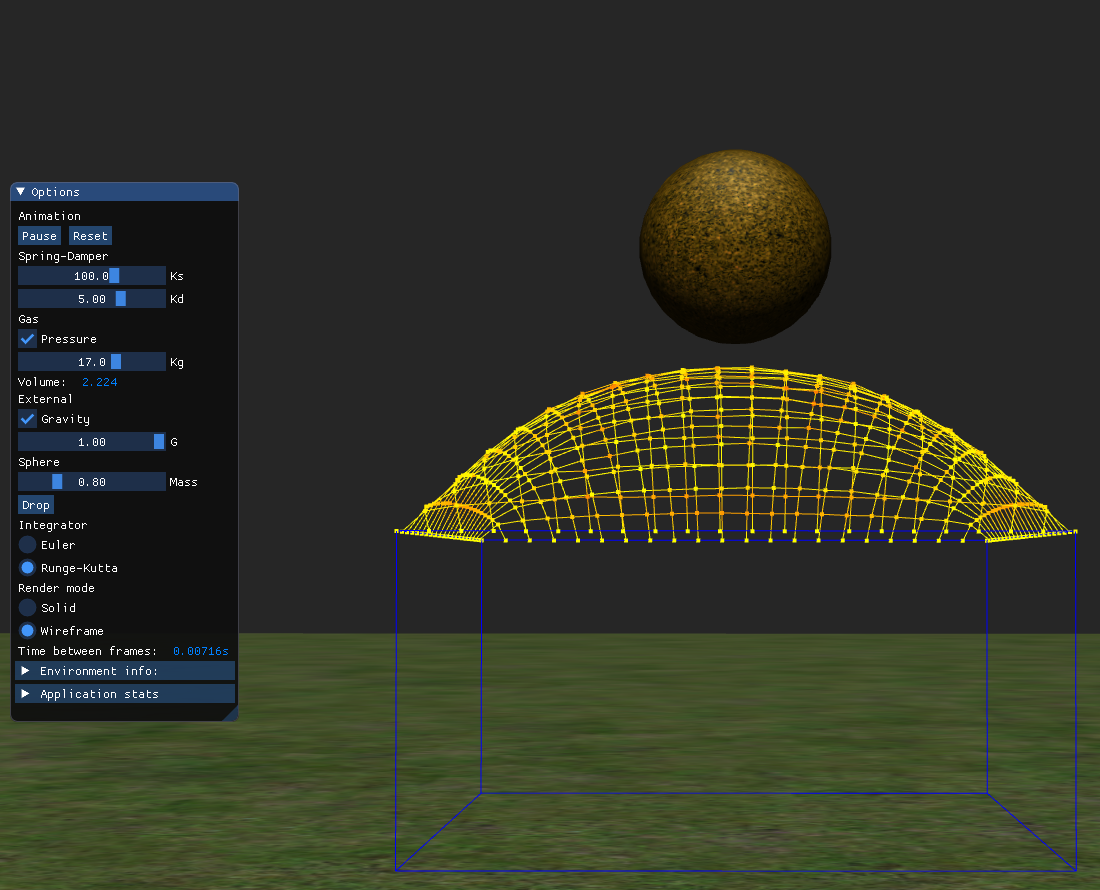
\includegraphics[width=\textwidth]{Img/04/positiveGravity1}
    \caption{La presión y la gravedad jalan la tela hacia arriba.}
    \label{fig:testGpos1}
  \end{subfigure}
~
  \begin{subfigure}[b]{0.45\textwidth}
    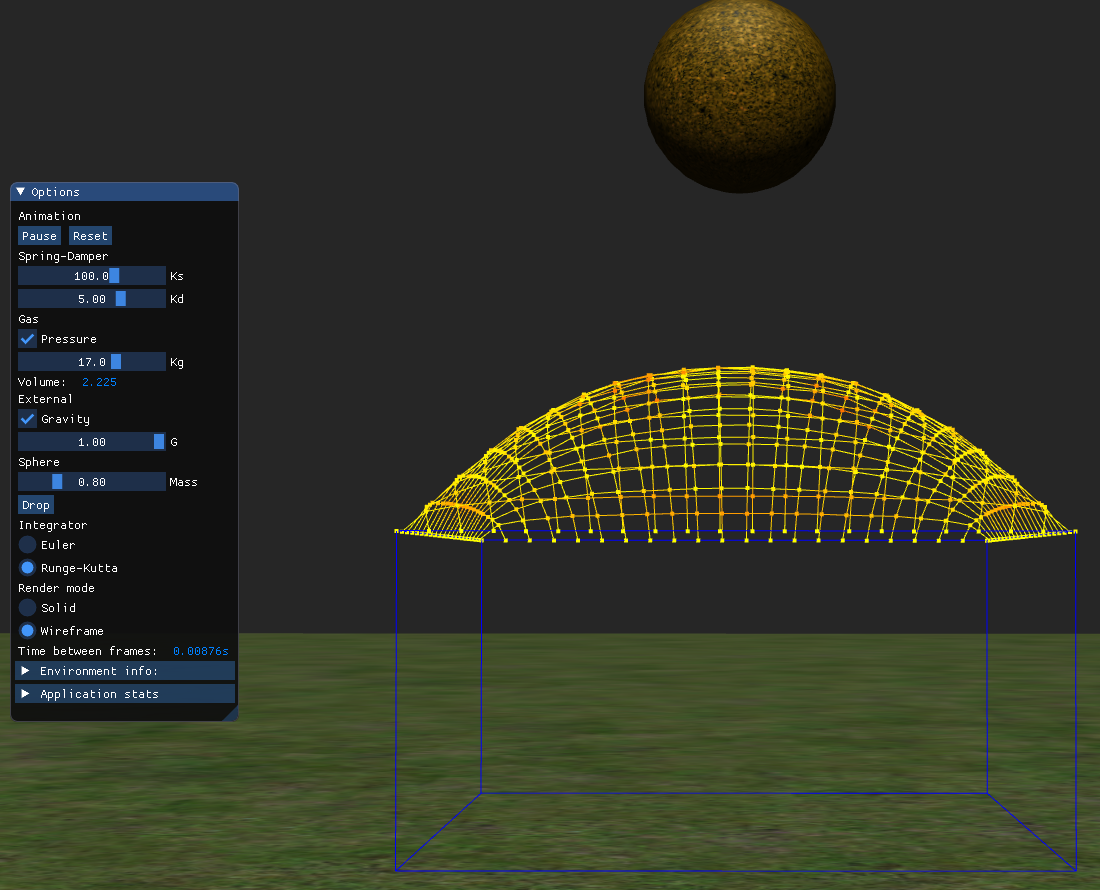
\includegraphics[width=\textwidth]{Img/04/positiveGravity2}
    \caption{La pelota también es jalada hacia arriba}
    \label{fig:testGpos2}
  \end{subfigure}
 \caption[Experimento: $g > 0$]{La fuerza de gravedad cambia de signo} 
 \label{fig:positiveGravity}
\end{figure}

Por último vamos a reiniciar la animación y partiendo de los valores de \emph{\textenglish{default}} de los parámetros, se apaga la gravedad. 
Este comportamiento equivale a hacer $g=0$ con la diferencia de que se hacen menos cálculos, ahora vemos cómo de nuevo la tela se mueve hacia arriba, cómo la gravedad se oponía a la fuerza del gas y ya no está, el gas empuja la tela aún más hacia arriba.
Si en esta situación se deja caer la pelota no pasará nada, debido a que la caída de la pelota \emph{depende de la gravedad}, y al no haber, simplemente no hay caída.

Si primero se deja caer la pelota sobre la tela, y una vez que ésta se estabiliza se apaga la gravedad, la pelota es empujada fuera del cuerpo flexible por un impulso.
Ver la Figura~\ref{fig:noGravity}.

\begin{figure}
 \centering
  \begin{subfigure}[b]{0.3\textwidth}
    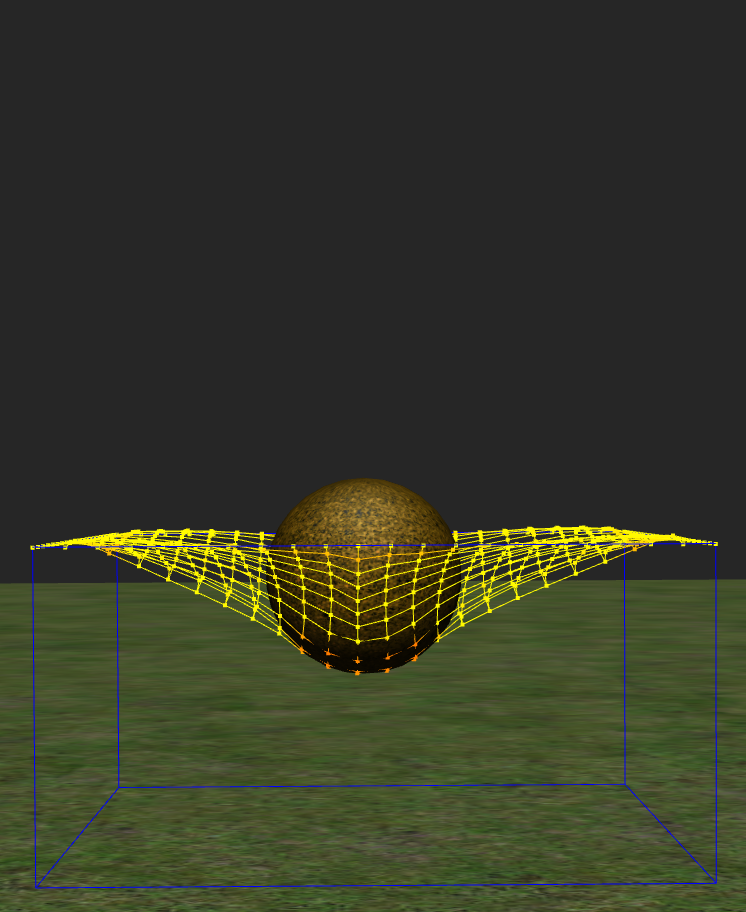
\includegraphics[width=\textwidth]{Img/04/gravityOff1}
  \end{subfigure}
~
  \begin{subfigure}[b]{0.3\textwidth}
    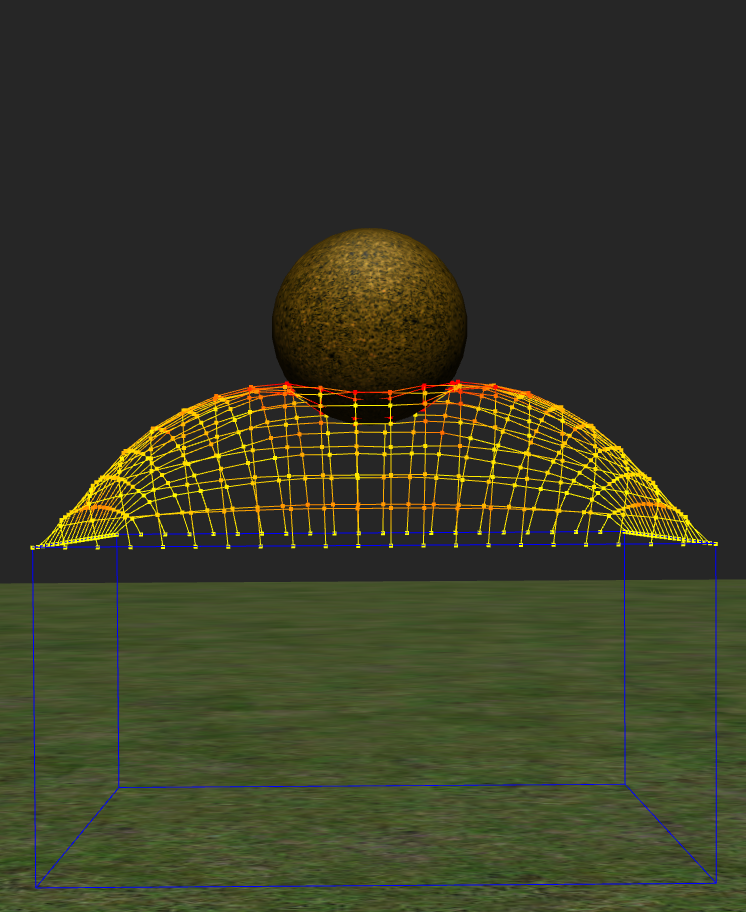
\includegraphics[width=\textwidth]{Img/04/gravityOff2}
  \end{subfigure}
~
  \begin{subfigure}[b]{0.3\textwidth}
    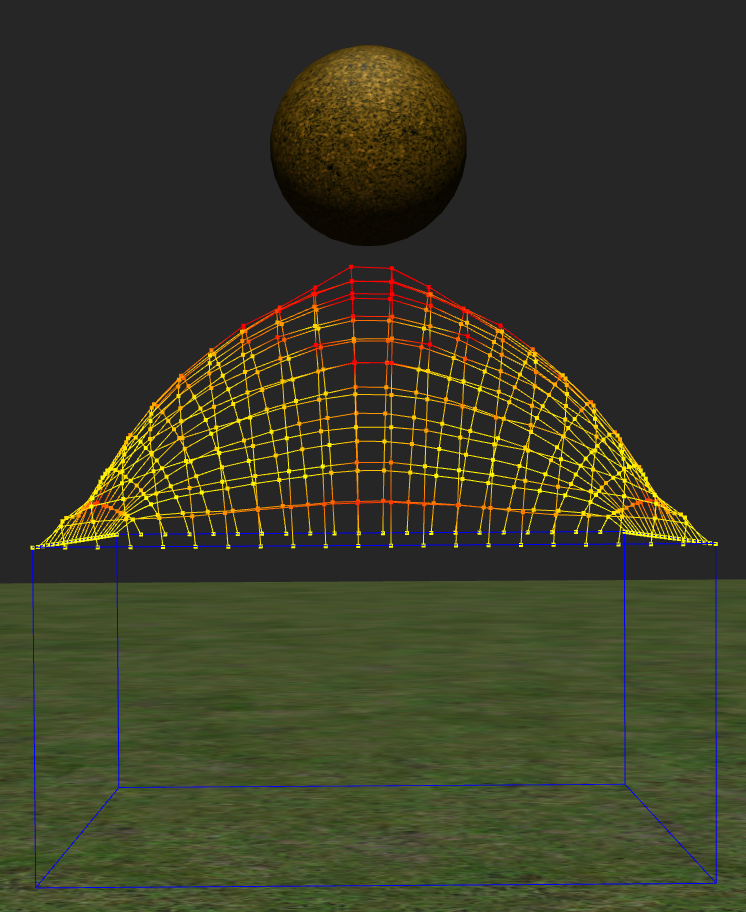
\includegraphics[width=\textwidth]{Img/04/gravityOff3}
  \end{subfigure}
 \caption[Experimento: Apagar la fuerza de gravedad]{La fuerza de gravedad es apagada después de que la pelota descansa sobre la tela.} 
 \label{fig:noGravity}
\end{figure}

\subsection{Probando la fuerza del gas}
Ahora se harán pruebas sobre la fuerza del gas. La fuerza del gas, por el diseño de nuestro experimento, se opone a la fuerza de gravedad, y actúa sólo sobre el cuerpo flexible.
Sin embargo, tiene cierto efecto sobre la velocidad de las partículas del cuerpo flexible, que a su vez tienen cierto efecto sobre el cuerpo \emph{rígido} cuando hay una colisión.

Inicie el programa con los valores de \emph{\textenglish{default}}, ahora apague la fuerza del gas y espere a que se estabilice el modelo, como se ve el la Figura~\ref{pres:test1}.
Como no hay fuerza del gas, la tela o cuerpo flexible cuelga agarrada de las orillas de la caja.
Ahora deje caer la pelota sobre el cuerpo flexible y espere a que se estabilice la animación, justo como se ve en la Figura~\ref{pres:test2}. 
Prenda la fuerza del gas y observe cómo la pelota es lanzada hacia arriba súbitamente como se ve en las Figuras~\ref{pres:test3} y~\ref{pres:test4}.

\begin{figure}
 \centering
  \begin{subfigure}[b]{0.45\textwidth}
    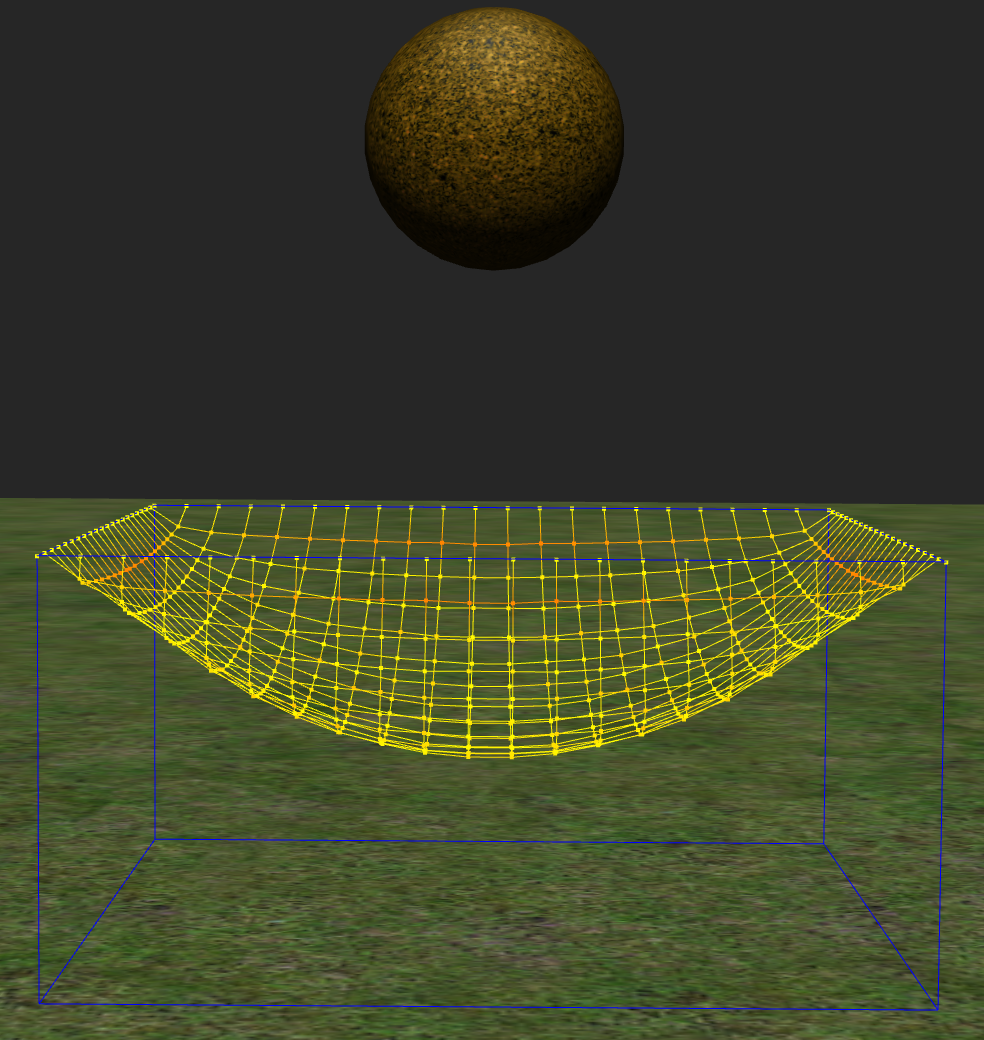
\includegraphics[width=\textwidth]{Img/04/modPress1}
    \caption{Fuerza del gas apagada}
    \label{pres:test1}
  \end{subfigure}
~
  \begin{subfigure}[b]{0.45\textwidth}
    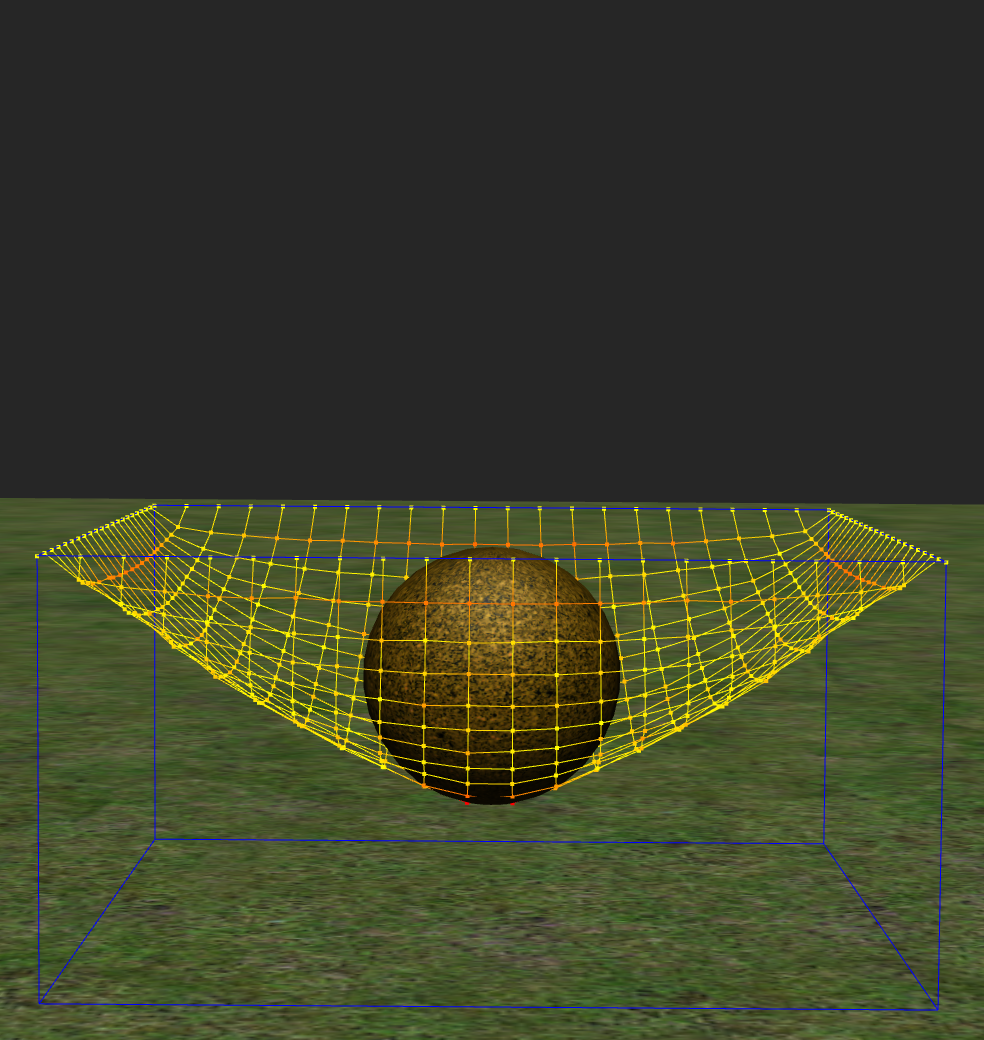
\includegraphics[width=\textwidth]{Img/04/modPress2}
    \caption{La pelota cae mientras está apagado el gas.}
    \label{pres:test2}
  \end{subfigure}
\\
  \begin{subfigure}[b]{0.45\textwidth}
    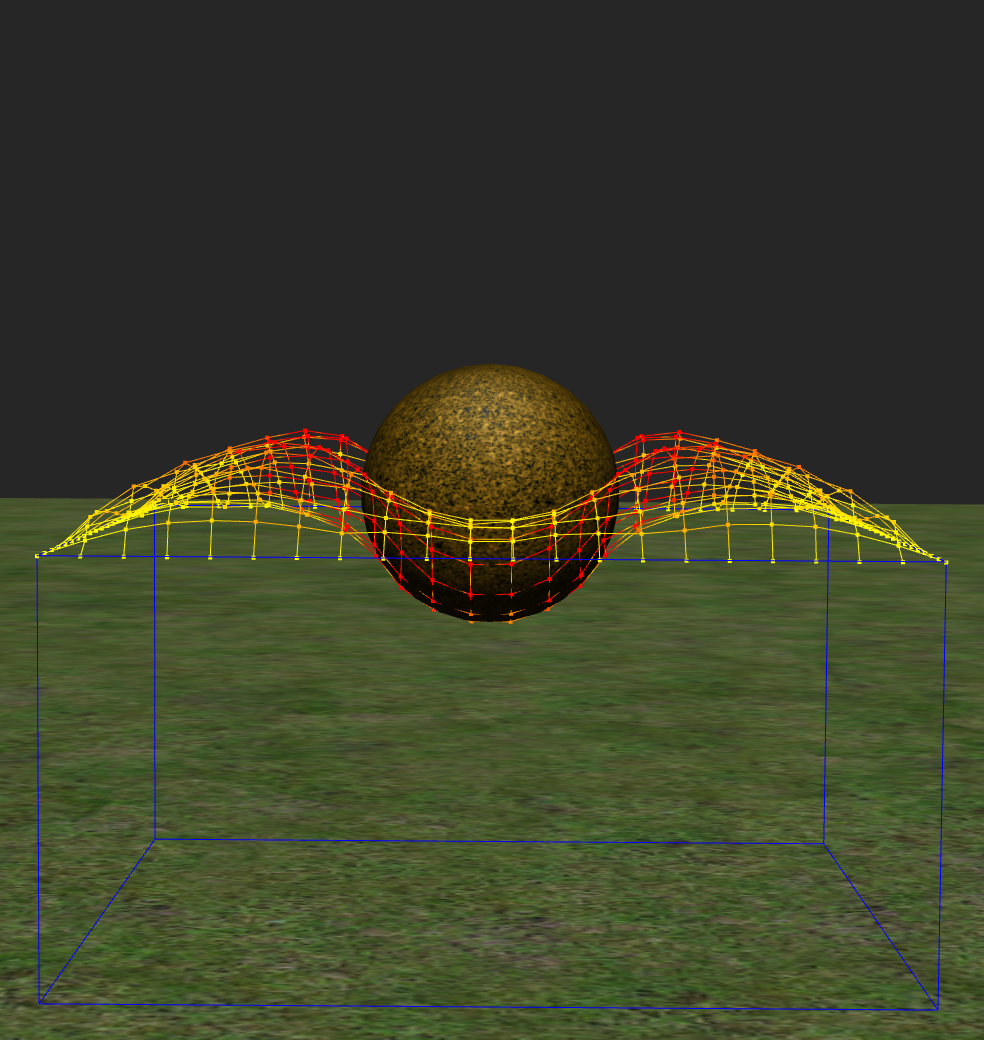
\includegraphics[width=\textwidth]{Img/04/modPress3}
    \caption{La fuerza del gas es encendida.}
    \label{pres:test3}
  \end{subfigure}
~
  \begin{subfigure}[b]{0.45\textwidth}
    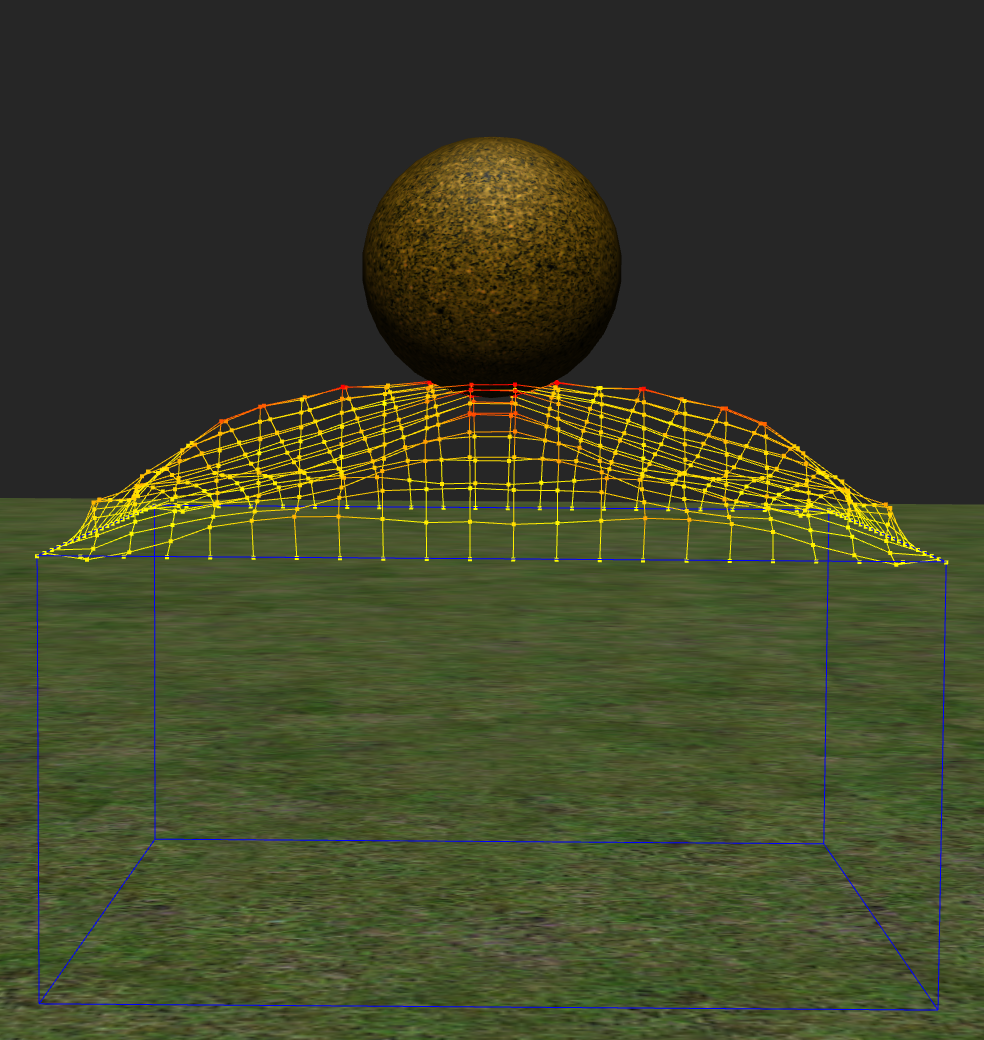
\includegraphics[width=\textwidth]{Img/04/modPress4}
    \caption{La pelota es lanzada por la fuerza del gas.}
    \label{pres:test4}
  \end{subfigure}
 \caption[Experimento: Fuerza del gas - cuerpo rígido]{La fuerza del gas interactúa con el cuerpo rígido.} 
 \label{pres:test}
\end{figure}

Otra prueba es ver los efectos de la variación de la constante $k_g$.
Inicie la animación con los valores de \emph{\textenglish{default}} y haga la constante $k_g$ pequeña, por ejemplo $k_g =11$; verá cómo el gas no es lo suficientemente fuerte para inflar el cuerpo flexible.
Ahora aumente poco a poco la constante $k_g$ y observe cómo se infla cada vez más el cuerpo flexible.
En la Figura~\ref{pres:testVar} se ilustran estas situaciones para diferentes valores en aumento de la constante $k_g$.

\begin{figure}
 \centering
  \begin{subfigure}[b]{0.30\textwidth}
    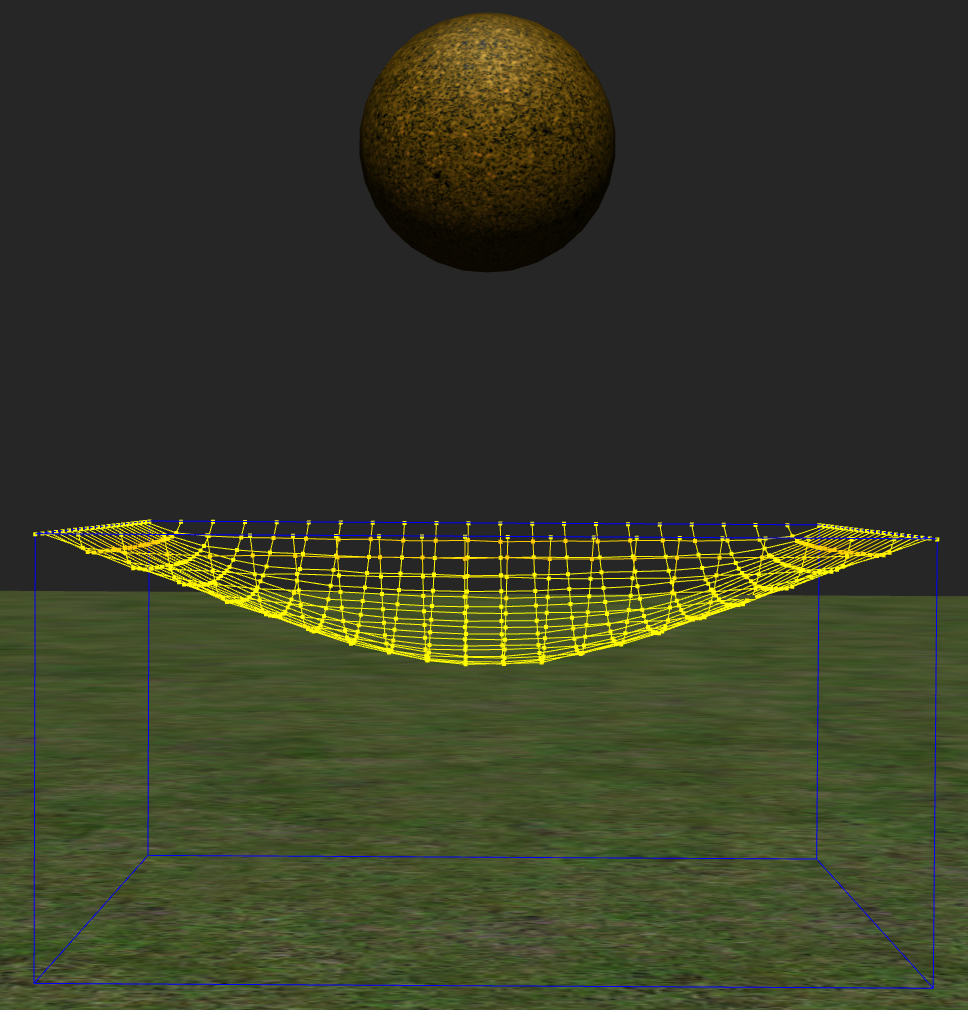
\includegraphics[width=\textwidth]{Img/04/varPress1}
    \caption{$k_g=11$.}
  \end{subfigure}
~
  \begin{subfigure}[b]{0.30\textwidth}
    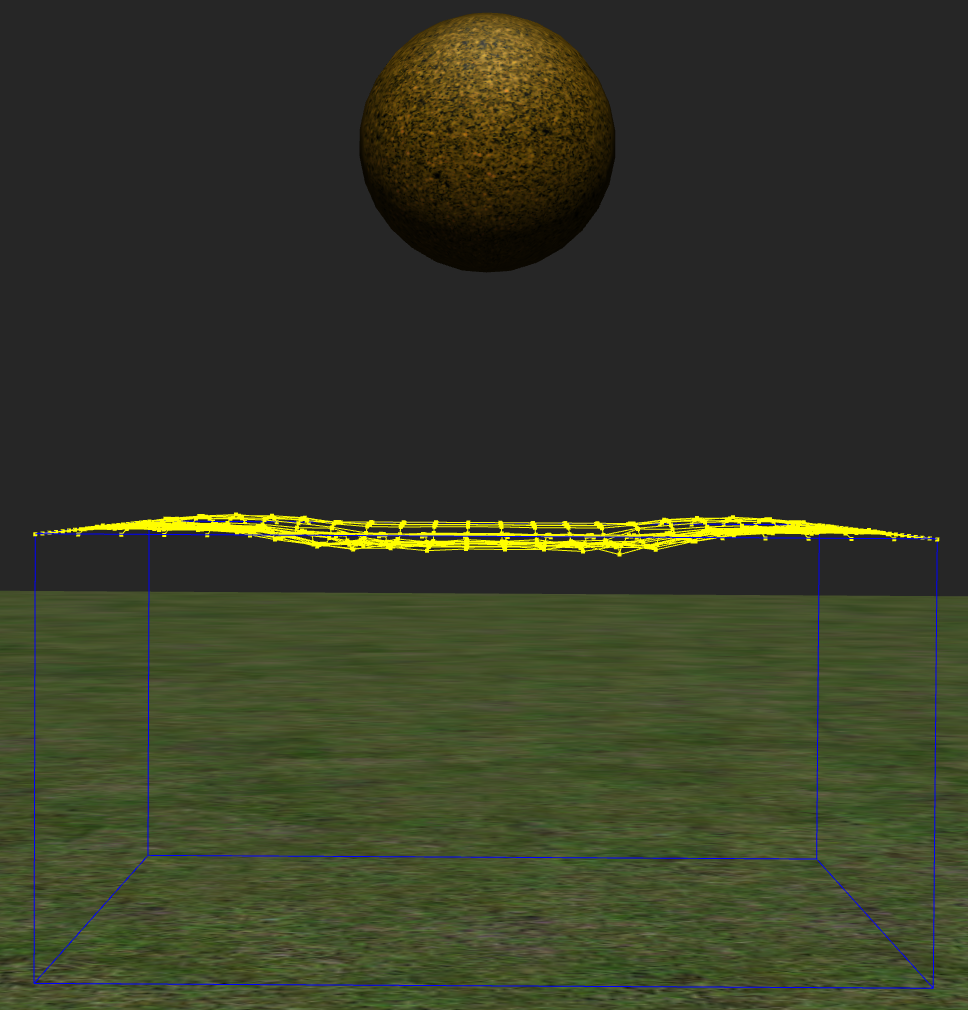
\includegraphics[width=\textwidth]{Img/04/varPress2}
    \caption{$k_g=17$.}
  \end{subfigure}
~
  \begin{subfigure}[b]{0.30\textwidth}
    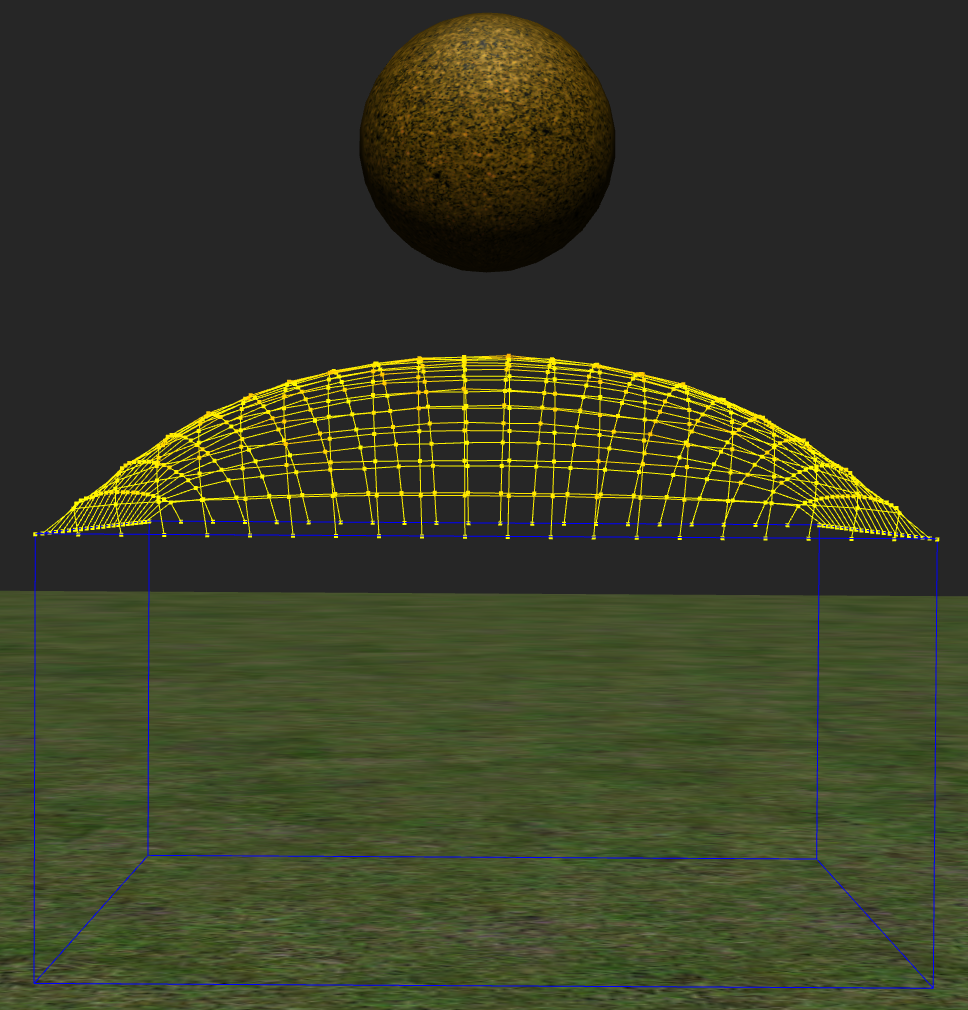
\includegraphics[width=\textwidth]{Img/04/varPress3}
    \caption{$k_g=25$.}
  \end{subfigure}
 \caption[Experimento: Variar la fuerza del gas]{El parámetro $k_g$ cambia la fuerza del gas.} 
 \label{pres:testVar}
\end{figure}

\subsection{Probando los resortes amortiguadores}
Las siguientes pruebas sirven para mostrar cómo funcionan los resortes amortiguadores.
Primero vamos a hacer una prueba con la constante de \emph{\textenglish{damping}} $k_d$.
Como ya se dijo, el damping es una forma de perder energía del sistema y, por lo tanto, de eventualmente estabilizarse.
Iniciemos la animación con los valores de \emph{\textenglish{default}} y hagamos la constante $k_d=0$, es decir quitemos todo el \emph{\textenglish{damping}}.
Vemos que la tela empieza a oscilar rápidamente como consecuencia del gas.
Ahora quitemos también el gas y esperemos un momento; veremos como la tela oscila sin detenerse ni estabilizarse en ningún momento, es cierto que cada vez oscila menos, pero ciertamente tardará mucho en detenerse (o nunca se detendrá).

En la Figura~\ref{res:test1}, podemos ver diferentes oscilaciones sin control por falta de un amortiguador.
Como ya se había dicho, el amortiguador agrega realismo (en la total ausencia de \emph{\textenglish{damping}}, el cuerpo flexible se ve poco real). La contra parte es que a mayor \emph{\textenglish{damping}}, también hay menos estabilidad numérica, por lo que el modelo es sumamente sensible al aumento en este parámetro.

\begin{figure}
 \centering
  \begin{subfigure}[b]{0.30\textwidth}
    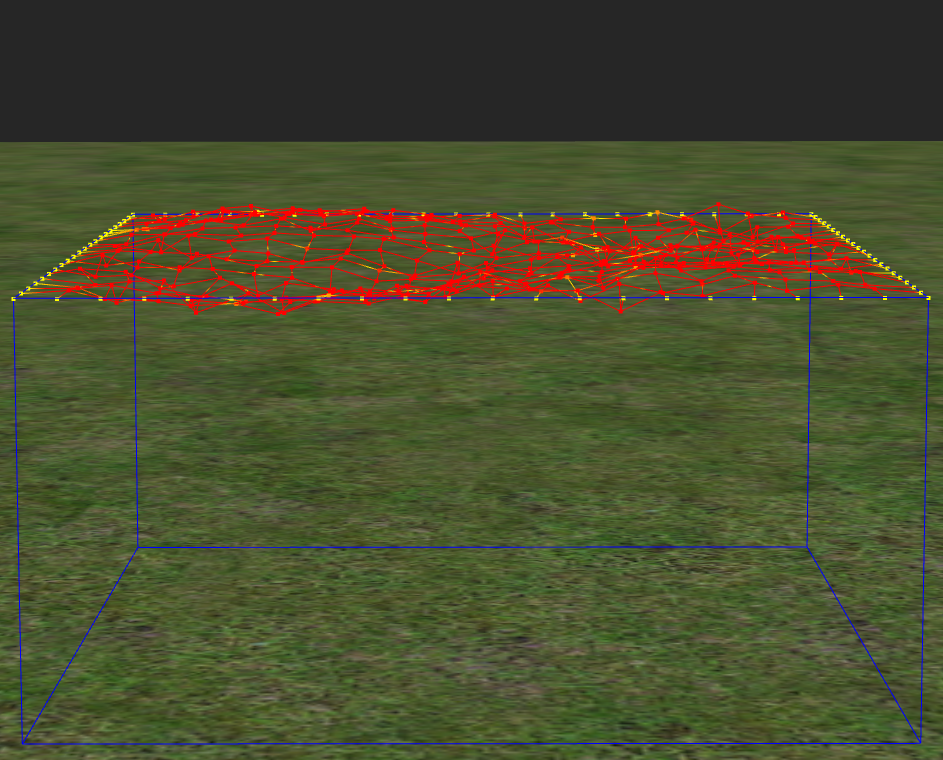
\includegraphics[width=\textwidth]{Img/04/noDamp1}
  \end{subfigure}
~
  \begin{subfigure}[b]{0.30\textwidth}
    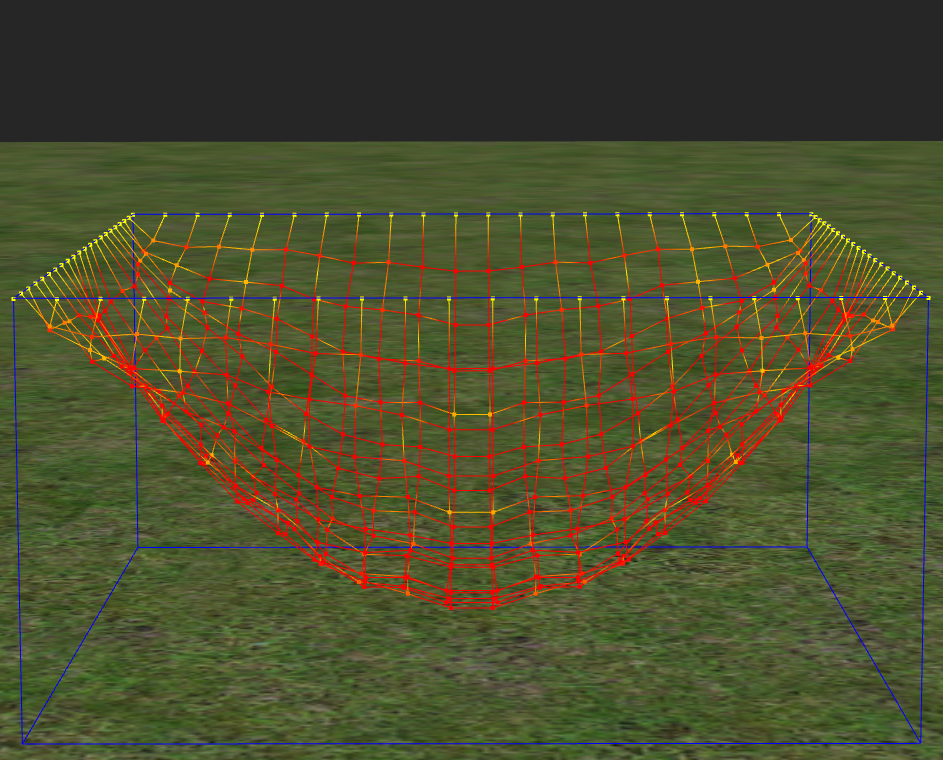
\includegraphics[width=\textwidth]{Img/04/noDamp2}
  \end{subfigure}
~
  \begin{subfigure}[b]{0.30\textwidth}
    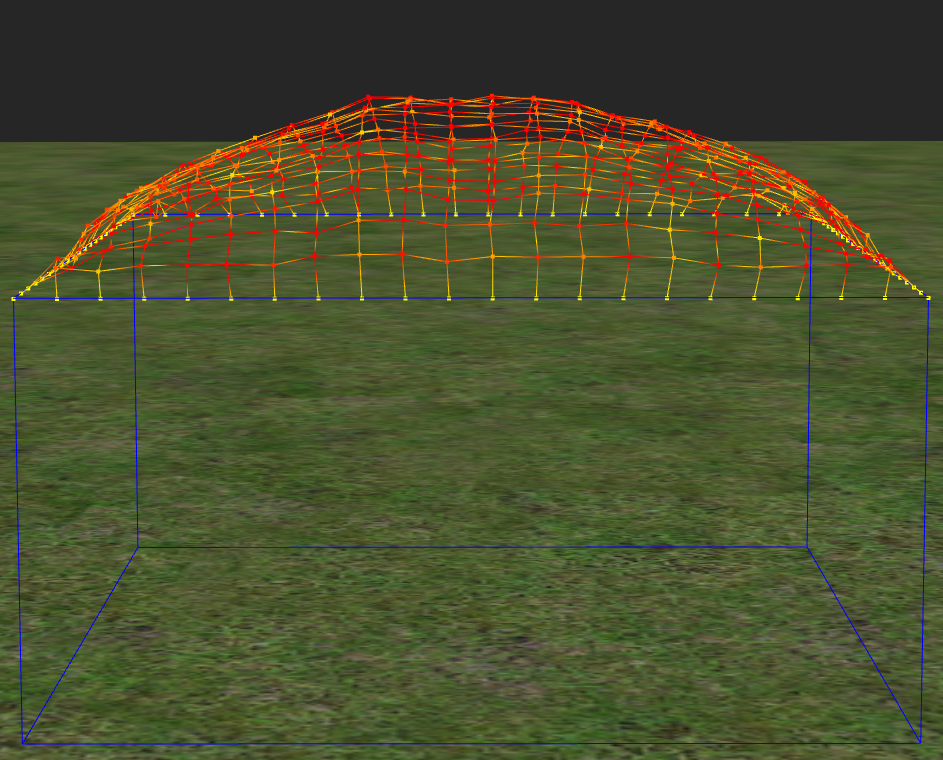
\includegraphics[width=\textwidth]{Img/04/noDamp3}
  \end{subfigure}
 \caption[Experimento: Quitar la fuerza del amortiguador]{Oscilación sin control: $k_d=0.0$} 
 \label{res:test1}
\end{figure}

Podemos ir aumentando el valor de $k_d$ poco a poco y ver cómo el modelo se vuelve inestable. 
Si se pone el máximo posible $k_d=7$ y se reinicia la animación, el modelo explota (ver Figura~\ref{res:test4}).

\begin{figure}
 \centering
 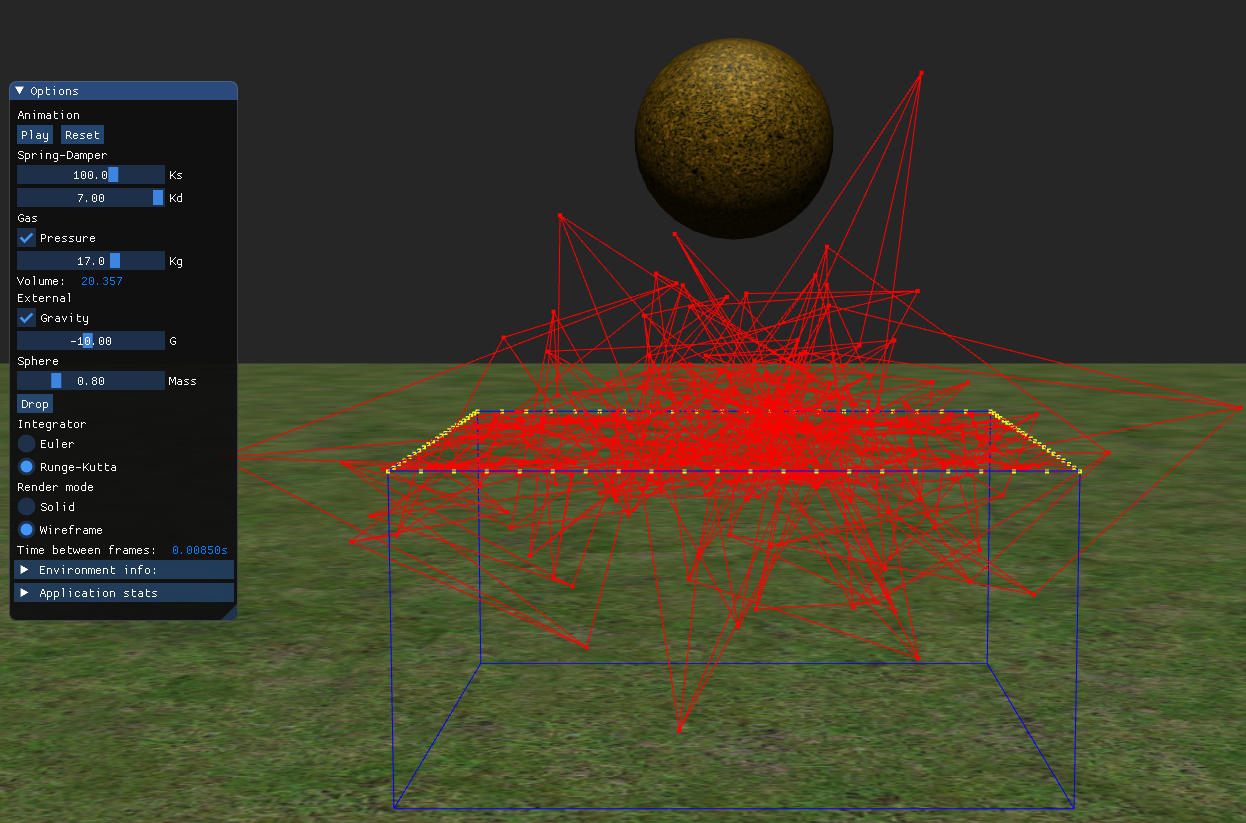
\includegraphics[width=0.85\textwidth]{Img/04/maxDamp}
 \caption[Explosión por inestabilidad numérica]{La animación explota por inestabilidad numérica}
 \label{res:test4}
\end{figure}

Ahora analicemos la constante de rigidez $k_s$.
Esta constante hace a los resortes más poderosos, por lo que en general hace que las partículas que están unidas por ellos, se separen menos, es decir hace más estable el cuerpo flexible en general, además de prevenir el efecto de super elongación.

Iniciamos la animación con los valores de default y pongamos la constante del resorte $k_s=200$ es decir a su máximo valor.
Ahora apaguemos el gas y vemos como la caída de la tela es menor, sin embargo al apagar y prender varias veces el gas también nos damos cuenta de que el cuerpo flexible parece oscilar más, como consecuencia de que los resortes en general jalan más fuerte, tanto hacia arriba como hacia abajo.

Ahora con la constante $k_g=17$, vayamos poco a poco subiendo la presión del gas. 
Podemos ver cómo aun con $k_g=17$, si $k_s=150$ el cuerpo flexible se expande poco; esperemos a que se estabilice, como se ve en la Figura~\ref{fig:maxRes1}. 
Ahora que tenemos el modelo estable y con $k_s$ máximo, poco a poco vayamos haciendo $k_s$ más pequeña y podremos apreciar cómo el cuerpo parece inflarse más (la resistencia de la membrana que lo mantiene unido es menor), como se ve en la Figura~\ref{fig:maxRes2}, hasta llegar al momento donde explota ($k_s$ = 0.0).

\begin{figure}
 \centering
  \begin{subfigure}[b]{0.45\textwidth}
    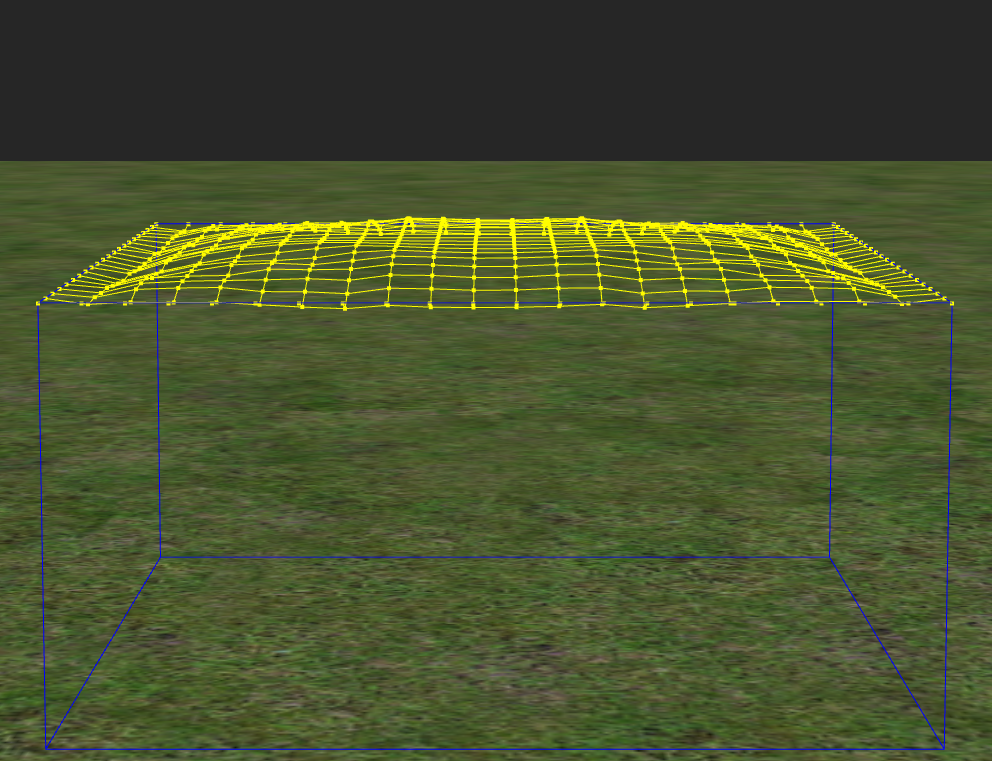
\includegraphics[width=\textwidth]{Img/04/maxRes1}
    \caption{Rigidez del resorte al máximo $k_s=150$}
    \label{fig:maxRes1}
  \end{subfigure}
~
  \begin{subfigure}[b]{0.45\textwidth}
    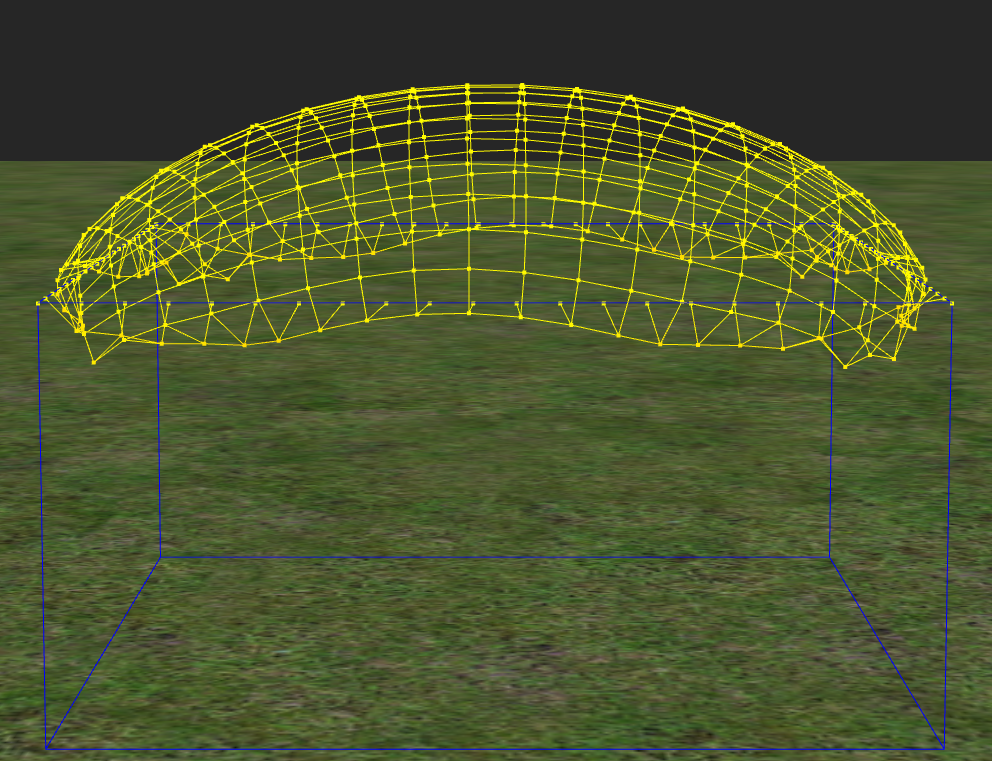
\includegraphics[width=\textwidth]{Img/04/maxRes2}
    \caption{La rigidez disminuye: $k_s=30$.}
    \label{fig:maxRes2}
  \end{subfigure}
 \caption[Experimento: Fuerza del resorte]{La fuerza del gas es constante a $k_g=17$ y variamos $k_s$} 
 \label{fig:maxRes}
\end{figure}

\section{Análisis del desempeño}

Una de las métricas más usadas para medir el desempeño de un programa gráfico es el número de veces que se actualiza el \emph{\textenglish{frame buffer}} en un segundo.
Está medida es conocida como \emph{fps} que es la abreviatura en ingles de  \emph{\textenglish{frames per second}}.
En general, es aceptado que para que una aplicación gráfica se considere en tiempo real (como debe ser un videojuego) se debe de alcanzar al menos 60 fps.

El programa es tan simple que aun en una tarjeta de video integrada en el CPU alcanza alrededor de 120 fps~\footnote{De hecho, cuando se ejecuta el programa usando la tarjeta de video Nvidia, el driver gráfico \emph{alenta} el programa para sincronizarse con la tasa de refresco del monitor. Es decir, al darse cuenta de que el programa produce frames más rápido de lo que los puede mostrar el hardware; hace el programa más lento para no desperdiciar recursos. Una tecnología conocida como \emph{\textenglish{vsync}}}
Por lo tanto, aunque esta medida es calculada (Figura~\ref{programa:menu}) en realidad nos dice muy poco del desempeño del programa.

Por esta razón, decidí utilizar el tiempo del proceso del CPU (medido en milisegundos) para hacer el análisis siguiente.

\subsection{Desempeño del programa}

Vamos a medir el tiempo que el CPU tarda en hacer todos los cálculos para producir un \emph{\textenglish{frame}}.
Vamos también a cronometrar el tiempo que toma procesar varias etapas del programa.
Tomando la primera medida como base, vamos a calcular la proporción del tiempo que es usado en cada etapa.

Decidí cronometrar las siguientes etapas:
\begin{description}
 \item[Tiempo entre frames:] La medida base. Este es el intervalo  de tiempo que toma hacer una iteración del ciclo principal del programa. Es decir el ciclo mostrado en la Figura~\ref{diagrama_flujo:fig}).
 \item[Tempor de \emph{\textenglish{render}}:] El tiempo que toma presentar al \emph{\textenglish{frame buffer}} una vez que se tienen los datos actualizados de todas las partículas y demás objetos de la escena al GPU. Es decir, el tiempo que toma la ejecución de todos los \emph{\textenglish{pipelines}} gráficos.
 \item[Tiempo de intergación:] Es el tiempo que toma calcular la posición y velocidad de cada partícula. En otras palabras el tiempo que toma ejecutar RK4.
 \item[Tiempo de manejo de colisiones:] El tiempo que toma ejecutar la detección y respuesta a las colisiones.
 \item[Tiempo de actualización de la malla:] El tiempo que toma primero recalcular las normales y después transmitir los datos completos (posiciones y normales de cada partícula) al GPU.
\end{description}

Adicionalmente, una parte del el \emph{tiempo de integración} es utilizado en evaluar la función fuerza.
Una evaluación si se integra con Euler, o cuatro evaluaciones si se integra con RK4.
Para ser más específicos y hacer un análisis parecido al anterior, se tomaron cuatro medidas además de la medida base.
Para la siguientes métricas se calcularon los tiempos totales que se pasa haciendo evaluaciones de cada parte de la función fuerza.
Es decir, que en el caso de que se integre con Euler es una medida, en el caso de que se integre con RK4 la suma de cuatro mediciones.

\begin{description}
 \item[Tiempo de evaluación de $F$:] La medida base. Este es el tiempo total que se pasó evaluando la función $F$ en cada frame.
 \item[Gravedad:] El tiempo total que tomó acumular la $F_g$ a todas las partículas.
 \item[Resortes:] El tiempo total que tomó acumular $F_s$ Y $F_d$ usando todos los resortes amortiguadores.
 \item[Volumen:] El tiempo total que se pasó calculando $V$, el volumen del cuerpo neumático. Este tiempo está contenido en el tiempo de presión.
 \item[Presión:] El tiempo total que se pasó acumulando $F_g$ recorriendo todas las caras.
\end{description}

Para hacer las mediciones se fijaron las siguientes condiciones:
Hacer render con caras sólidas y texturas.
Utilizar el método de RK4 para integrar.
Dejar caer la pelota sobre la tela para forzar que haya colisiones en cada frame.
Desde luego, que los tiempos anteriores son diferentes para cada frame.
Por esta razón se decidió ejecutar el programa y registrar los tiempos de cada frame de la ejecución.

Se registraron alrededor de 3200 frames.
Como primer método de exploración de los datos se presenta el \emph{resumen de 5 números} de cada una de las categorías.
El resumen de cinco números nos ayuda a ver que tanta dispersión hay entre los datos y que forma puede tener la distribución.
Está formado por cinco estadísticos: El mínimo de los datos ($\min$), el primer cuartil ($Q_1$), la mediana ($\tilde{x}$), el tercer cuartil ($Q_3$) y el máximo de los datos ($\max$).

\begin{table}
\ra{1.2}
\begin{center}
\begin{tabular} {@{}lrrrrr@{}}
\toprule
 & Render & Integración & Colisión & Malla & Frame \\
\midrule 
 $\min$      &  0.2533 &  2.2235 & 0.0257 & 0.3272 &  3.1157 \\
 $Q_1$       &  0.9312 &  2.6941 & 0.0325 & 0.3957 &  6.3076 \\
 $\tilde{x}$ &  2.9606 &  3.7973 & 0.0442 & 0.5198 &  7.5509 \\
 $Q_3$       &  5.1519 &  5.1556 & 0.0572 & 0.6769 &  8.3865 \\
 $\max$      & 26.8164 & 12.3506 & 0.1548 & 1.7716 & 30.3281 \\
\bottomrule
\end{tabular}
\end{center}
\caption[Resumen de medidas por frame]{Resumen de cinco números de las medidas para calcular un frame.}
\label{resumenFrame:tabla}
\end{table}

\begin{table}
\ra{1.2}
\begin{center}
\begin{tabular} {@{}lrrrrr@{}}
\toprule
 & Gravedad & Resortes & Volumen & Presión & $F$ \\
\midrule 
 $\min$      & 0.0383 & 0.5527 & 0.3331 & 1.3756 &  1.9747 \\
 $Q_1$       & 0.0475 & 0.6788 & 0.4072 & 1.6615 &  2.3912 \\
 $\tilde{x}$ & 0.0677 & 0.9531 & 0.5679 & 2.3528 &  3.3860 \\
 $Q_3$       & 0.0950 & 1.3141 & 0.7834 & 3.2024 &  4.6050 \\
 $\max$      & 0.2386 & 3.1087 & 1.9180 & 7.7122 & 11.0151 \\
\bottomrule
\end{tabular}
\end{center}
\caption[Resumen de medidas de evaluación de $F$]{Resumen de cinco números de las medidas relativas a la evaluación de $F$.}
\label{resumenFuerza:tabla}
\end{table}

Como puede verse en el Cuadro~\ref{resumenFrame:tabla} y en el Cuadro~\ref{resumenFuerza:tabla} hay algunos \emph{\textenglish{outliers}} en la parte alta de los datos.
Ambas distribuciones están sesgadas a la derecha.
Esto quiere decir que hay algunos frames particularmente lentos~\footnote{Esto es común en los programas gráficos, un frame puede ser inusualmente lento por varias razones. Por ejemplo: si la ventana cambio de tamaño (y hubo que recrear el \emph{\textenglish{frambuffer}}), si hubo un cambio en el modo de \emph{\textenglish{render}} (y hubo que recrear el \emph{\textenglish{pipeline}} gráfico) o si hubo que cambiar \emph{\textenglish{assets}} (y hay que actualizar la memoria de video)}.

Sin embargo, en realidad los datos no están tan dispersos pues las distancias entre los $Q_1$ y $Q_3$ es proporcionalmente pequeña en todos los casos.
Con esto en mente, decidí tomar la media aritmética ($\bar{x}$); mejor conocida como el \emph{promedio}, de cada medida para poder hacer el cálculo que nos interesa.

Para calcular la proporción que cada medida representa con respecto de la medida base, simplemente dividí el promedio de la medida entre el promedio de la medida base y lo multiplique por 100 (Para expresarlo en forma de porcentaje)


\begin{table}
\ra{1.2}
\begin{center}
\begin{tabular} {@{}lrrrrr@{}}
\toprule
 & Render & Integración & Colisión & Malla & Frame \\
\midrule 
 $\bar{x}$      & 3.0502 & 4.4734 & 0.0498 & 0.5878 & 8.2945 \\
 $\%$           & 36.77 & 53.93 & 0.60 & 7.09 & \\
\bottomrule
\end{tabular}
\end{center}
\caption[Proporción de cálculos por frame]{Proporción de tiempo de los cálculos con respecto a un frame.}
\label{propFrame:tabla}
\end{table}

Hay algunos datos interesantes en el Cuadro~\ref{propFrame:tabla}.
Como se esperaba, la rutina computacionalmente más demandante es el método numérico, con cerca del $54\%$ del tiempo.
Resalta también que el manejo de las colisiones es casi insignificante pues no alcanza ni siquiera un $1\%$.
Esto puede deberse a que en realidad el número de partículas es pequeño y la detección entre punto y esfera es muy sencilla.

Finalmente, quiero señalar que dado que hay más operaciones que no se midieron.
El manejo de la interacción con el usuario es uno, por dar un ejemplo.
Por esa razón, la suma de los componentes no da el $100\%$ del tiempo para producir un frame.

\begin{table}
\ra{1.2}
\begin{center}
\begin{tabular} {@{}lrrrrr@{}}
\toprule
& Gravedad & Resortes & Volumen & Presión & $F$ \\ 
\midrule 
 $\bar{x}$      & 0.0803 & 1.1376 & 0.6796 & 2.7712 & 3.9920 \\
 $\%$           & 2.01 & 28.50 & 17.02 & 69.42 & \\
\bottomrule
\end{tabular}
\end{center}
\caption[Proporción de cálculos de $F$]{Proporción de tiempo de los cálculos con respecto a la evaluación de $F$.}
\label{propFuerza:tabla}
\end{table}

Con respecto al Cuadro~\ref{propFuerza:tabla} vemos que el cálculo de la $F_g$ es el más costoso con el $70\%$ del tiempo.
Seguido de los cálculos de $F_s$ y $F_d$ con el $28.5\%$.
La acumulación de $G$ es casi despreciable.
Esto quiere decir, que el tiempo de cálculo es directamente proporcional al número de partículas involucradas.
Hay \emph{una} partícula involucrada para acumular $G$, \emph{dos} para acumular $F_s$ y $F_d$ y \emph{cuatro} para acumular $F_g$.
Sin mencionar, que para calcular $F_g$, primero debemos calcular $V$.

El tiempo de cálculo de $V$ forma parte del tiempo de cálculo de $F_g$.
De hecho, del $69\%$ de tiempo que ocupamos en calcular $F_g$, el cálculo de $V$ aporta un $17\%$ (casi una cuarta parte).
Es por esta razón que si se suman los porcentajes de gravedad, resortes y presión casi se da el total para producir $F$.

Por último hago énfasis en que aún cuando cada experimento con del programa arrojará datos diferentes, las proporciones reportadas en el Cuadro~\ref{propFrame:tabla} y el  Cuadro~\ref{propFuerza:tabla} tienden a ser \emph{casi} las mismas.
Puede volverse a mirar la Figura~\ref{programa:menu} que se capturó con otra ejecución del programa y también reporta proporciones parecidas.
Mas aún, cualquier implementación que siga los algoritmos descritos en éste trabajo \emph{deberá} presentar proporciones muy similares en los cálculos.
Por lo tanto, los datos en los Cuadros ~\ref{propFrame:tabla} y~\ref{propFuerza:tabla} son una aportación relevante de ésta tesis.
